\section{Ячейка Фейстеля}\index{ячейка Фейстеля|(}
\selectlanguage{russian}

Следующей идеей, продвинувшей развитие блочных шифров и приведшей к появлению государственного стандарта DES\index{шифр!DES}, стало появление конструкции, получившей название \emph{ячейка Фейстеля}. Данная конструкция приведена на рис.~\ref{fig:Feistel}.

\begin{figure}[!htb]
    \centering
    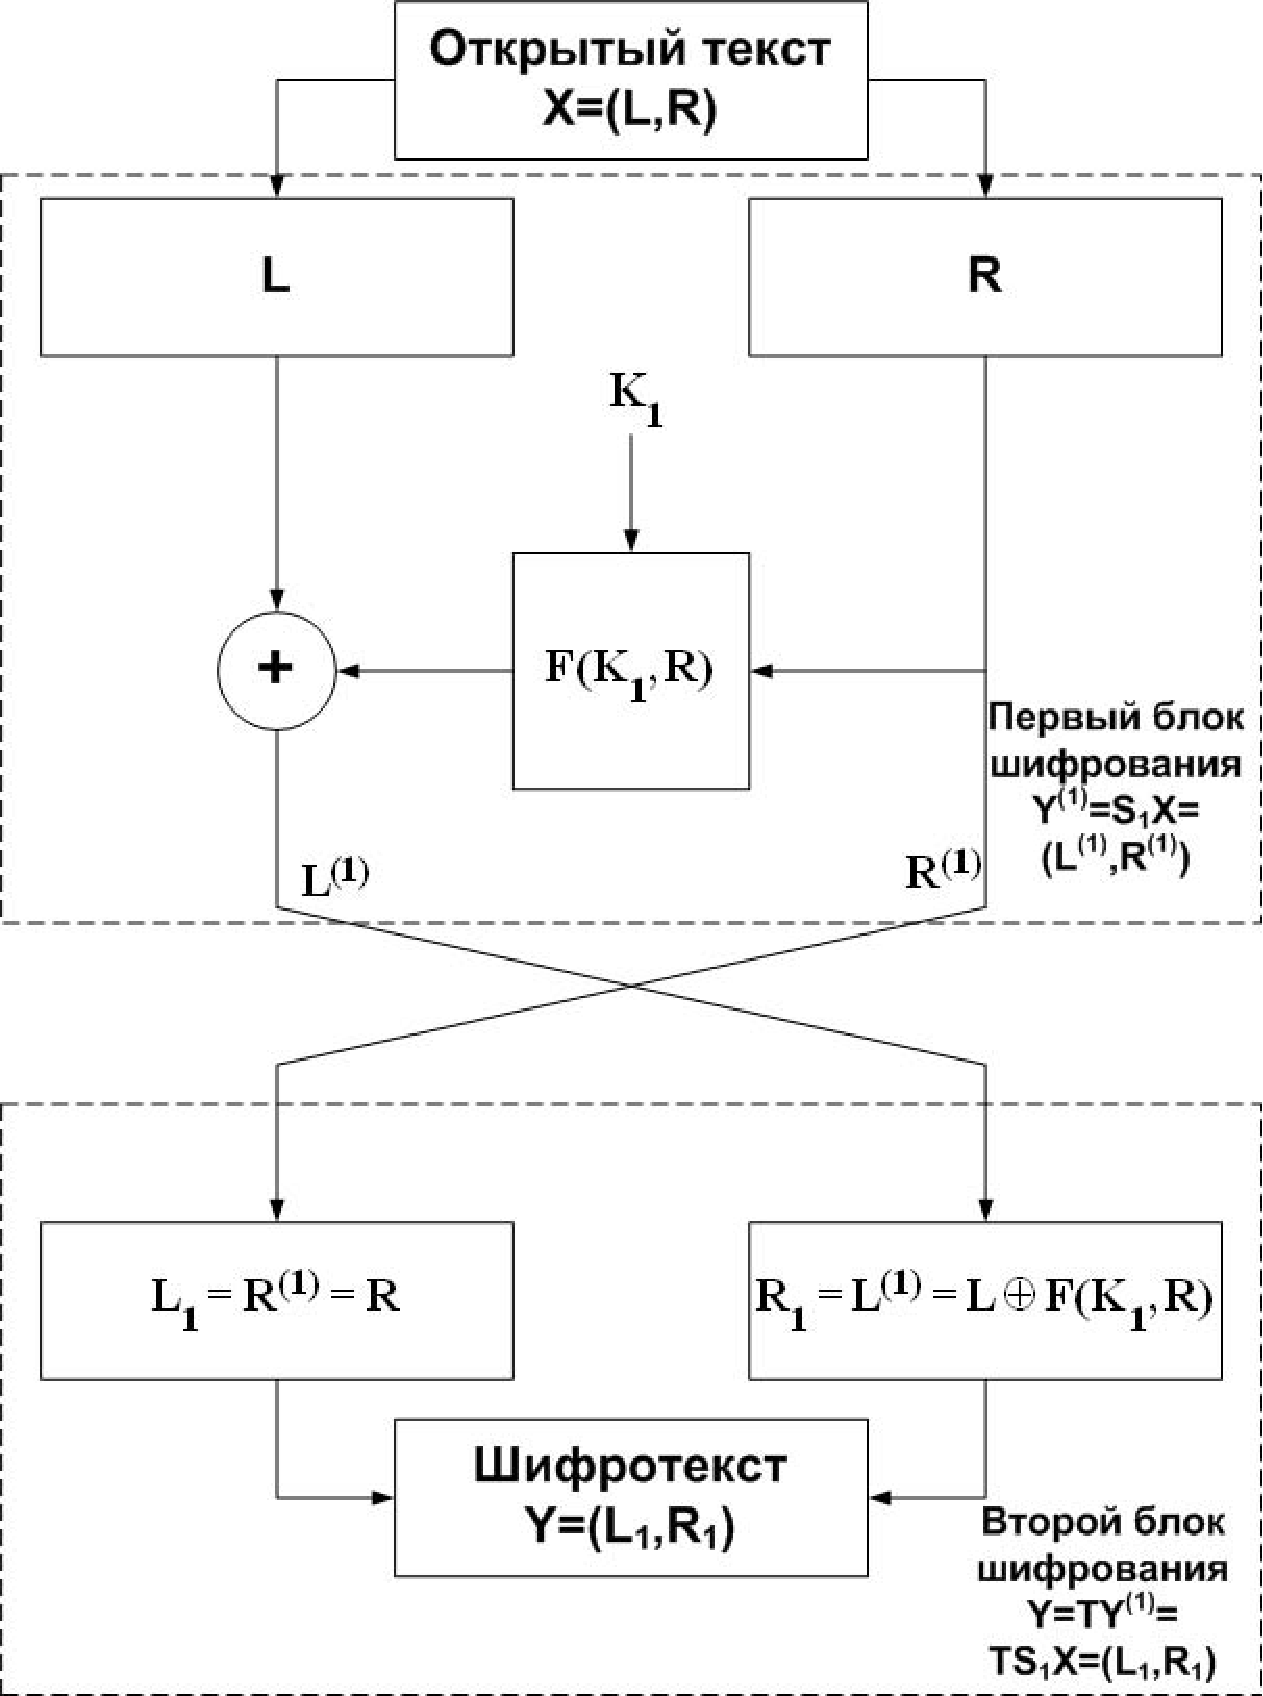
\includegraphics[width=0.6\textwidth]{pic/feistel}
    \caption{Ячейка Фейстеля\label{fig:Feistel}}
\end{figure}

На рисунке~\ref{fig:Feistel} изображён один раунд шифрования блочного шифра, использующего оригинальную ячейку Фейстеля. Каждый раунд шифрования принимает на вход блок с чётным количеством бит и делит его на две равные части $L_k$ и $R_k$. Входным блоком для первого раунда является блок открытого текста. Правая часть $R_k$ без изменений становится левой частью входного блока $L_{k+1}$ следующего раунда шифрования. Кроме того, правая часть подаётся на вход \emph{функции Фейстеля} $F\left(R_k, K_k \right)$\index{функция!Фейстеля}, аргументами которой являются половина блока данных и раундовый ключ\index{ключ!раундовый} (раундовые ключи получаются в результате работы алгоритма ключевого расписания, как описано в разделе~\ref{section-block-ciphers-intro}). Результат работы функции Фейстеля складывается с помощью побитового сложения по модулю 2 с левой частью входного блока $L_k$. Полученная последовательность бит становится правой частью выходного блока раунда шифрования. Таким образом, работа $k$-ого раунда ячейки Фейстеля описывается следующими соотношениями:

\[\begin{array}{l}
    L_{k+1} = R_{k}, \\
    R_{k+1} = L_{k} \oplus F\left( R_k, K_k \right).
\end{array}\]

Результатом шифрования является конкатенацией последних выходных блоков $L_n$ и $R_n$, где $n$ -- число раундов шифрования.

Несложно показать, что, зная раундовые ключи $K_1, \dots, K_n$ и результат шифрования $L_n$ и $R_n$, можно восстановить открытый текст. В частности, для каждого раунда:
\[\begin{array}{l}
    R_k = L_{k+1}, \\
    L_k = R_{k+1} \oplus F\left( R_k, K_k \right).
\end{array}\]

Таким образом, ячейка Фейстеля гарантирует корректность работы блочного шифра вне зависимости от сложности функции Фейстеля\index{функция!Фейстеля} $F\left(R_k, K_k \right)$. В результате криптограф (автор шифра) при использовании ячейки Фейстеля не должен беспокоиться об обратимости функции шифрования в целом (конструкция ячейки Фестеля уже гарантирует это), а должен беспокоиться только о достаточной криптографической стойкости функции Фейстеля, необратимость которой не требуется (и даже вредит криптостойкости). Функция Фейстеля обычно состоит из блоков перестановки и подстановки бит (то есть из p- и s-блоков, уже рассмотренных ранее).

\index{ячейка Фейстеля|)}
